\documentclass[11pt,a4paper]{article}

% ---- packages ----
\usepackage[margin=1in]{geometry}
\usepackage{amsmath,amssymb,amsthm}
\usepackage{booktabs}
\usepackage{graphicx}
\usepackage{hyperref}
\usepackage{url}
\usepackage{xcolor}
\usepackage{enumitem}
\usepackage{microtype}
\usepackage[T1]{fontenc}
\usepackage{lmodern}

\hypersetup{
  colorlinks=true,
  linkcolor=blue!50!black,
  citecolor=blue!50!black,
  urlcolor=blue!60!black
}

\title{Formally Verified Parameter-Free Scalar Engine\\
for Contested Cosmology:\\
Lean~4 and Multi-Prover Certification of\\
Fluid Spacetime Omni-Theory}

\author{Damian Arthur Palumbo\\
\textit{Independent researcher}\\[0.6em]
\texttt{https://github.com/dappalumbo91/FSOT-2.1-Lean}}

\date{Edition freeze 2026-07-16 \quad Manuscript 2026-07-31}

\begin{document}
\maketitle

\begin{abstract}
Modern physics is accurate in fragments and fragmented in architecture.
Sector models accumulate free parameters, and contested observables---especially
the Hubble constant $H_0$ dual-anchor tension---expose the cost.
We present a machine-checked, zero free-parameter scalar engine for
Fluid Spacetime Omni-Theory (FSOT): a seed-derived vitality scalar
$\mathrm{raw}\_S=\mathrm{term}_1+\mathrm{term}_2+\mathrm{term}_3$
built only from $\pi$, $e$, $\varphi$, $\gamma$ (Euler--Mascheroni), and
Catalan's $G$, with domain routes as preregistered folds rather than
per-observable least-squares knobs.

Formally, the edition freeze reports
\mbox{\texttt{overall\_ok: true}}
for \textbf{1{,}863} atomic obligations (Lean~4 primary authority; export to
Coq/Rocq, Isabelle/HOL, F$^*$, and Rust executable replay), bound to a
SHA-256-pinned Python oracle.
Empirically, contested-sector pooled median error is \textbf{0.030\%}
across 13 monitored observables (dual-anchor $H_0$, $\sigma_8$, BBN lithium
proxy, hierarchy, $w_a$), versus a $\sim$15\% typical baseline tension scale
for open $\Lambda$CDM/SM panels.
Dual-anchor $H_0$ uses a bubble-bleed route ($\mathrm{term}_3$ turbulence with
$\mathrm{perceived\_adjust}$ on $\mathrm{term}_1$); preregistered PRED-001 places
the FSOT bridge scalar strictly between Planck 2018 CMB and Riess et~al.\ local
anchors.

We scope this paper to the formal spine and contested cosmology---not a
400-domain monograph.
The full 402-domain atlas (536{,}740 records; 394/394 domains under a
$\le 0.5\%$ green gate) is the living GitHub thesis.
Readers can accept or reject claims by running the published verification bundle.
\end{abstract}

\noindent\textbf{Keywords:}
formal methods; Lean~4; multi-prover verification; parameter-free models;
Hubble tension; Fluid Spacetime Omni-Theory; reproducible science.

\vspace{0.8em}
\noindent
\begin{center}
\begin{minipage}{0.95\linewidth}
\hrule\vspace{0.5em}
{\small
\textbf{Software availability (required).}
Lean~4 formalization, five-prover obligation export, Python decimal oracle
(\texttt{vendor/fsot\_compute.py}), contested-sector ledger, preregistered
predictions PRED-001--041, and one-command verification.

\centering
\url{https://github.com/dappalumbo91/FSOT-2.1-Lean}

\smallskip
Recommended checkout: tag \texttt{v2.6-arxiv-paper01} (commit \texttt{8a44947};
includes \texttt{matplotlib} in \texttt{requirements.txt}).\\
Oracle SHA-256:
\texttt{D1D38A185487B452E470AC68ECE2EB45AEB1CA9CE25FC9BF9564C19633FFBE70}.

\begin{verbatim}
git clone https://github.com/dappalumbo91/FSOT-2.1-Lean.git
cd FSOT-2.1-Lean
# tip includes matplotlib>=3.8 in requirements.txt (commit 8a44947+)
pip install -r requirements.txt
python scripts/run_publication_verification_bundle.py
\end{verbatim}

\noindent Full five-prover path:
\texttt{python scripts/run\_publication\_verification\_bundle.py --full-cross-proof}.
Independent freeze check (paper package):
\texttt{python verify\_paper\_claims.py --fsot-root . --strict-hash}.
Cosmology navigation:
\texttt{python scripts/query\_fsot\_domain\_navigator.py --intent cosmology\_cmb}.
}
\vspace{0.5em}\hrule
\end{minipage}
\end{center}

\section{Introduction}
\label{sec:intro}

\subsection{The fragmentation problem}

Twentieth-century physics delivered extraordinary local theories---general
relativity, quantum mechanics, the Standard Model, and $\Lambda$CDM
cosmology---each optimized inside institutional and mathematical boundaries.
The empirical cost appears where boundaries meet: parameter proliferation,
cross-sector tension (local $H_0$ versus CMB inference
\cite{Planck2018,Riess2022,Riess2024}), siloed success, and unified narratives
without executable kill criteria.

$\Lambda$CDM explains CMB and large-scale structure with excellent
\emph{internal} consistency, yet the $H_0$ and $\sigma_8$ tensions remain open
scientific problems \cite{Planck2018,Riess2022,DESY3,PoulinEDE}.
FSOT does not reject those \emph{data}.
It rejects the architecture: many knobs, many silos, no single engine that must
survive formal and empirical gates at once.

\subsection{Operational claim}

\begin{quote}
Reality is modeled as a 25-dimensional fluid condensate.
Observed regimes of space, time, matter, and measurement are folds of a single
scalar field $\mathrm{raw}\_S$, computed from seed geometry with
\textbf{no per-observable least-squares tuning}.
\end{quote}

Routing coordinates $(D_{\mathrm{eff}},\delta\psi,\mathrm{recent\_hits},
\mathrm{observed})$ are declared in domain manifests before comparison; failed
green gates are ledger events, not silent parameter rescues.

\subsection{Formal methods as scientific instruments}

Proof assistants are standard in software verification; their use as
\emph{scientific instruments} is growing (formal chemical theory
\cite{Bobbin2024}; HepLean for high-energy physics \cite{HepLean2024}).
Numeric scripts alone can drift.
FSOT answers with: Lean~4 primary formalization; Coq/Rocq, Isabelle/HOL, F$^*$,
and Rust export; a hash-locked Python oracle; and preregistered predictions
PRED-001--041.

\subsection{Scope}

Following the scope discipline of HepLean (selected HEP areas)
\cite{HepLean2024} and Bobbin et~al.\ (selected classical theories)
\cite{Bobbin2024}, this paper is \textbf{focused}:

\begin{center}
\begin{tabular}{@{}p{0.45\linewidth}p{0.45\linewidth}@{}}
\toprule
\textbf{In scope} & \textbf{Out of main body (GitHub thesis)} \\
\midrule
Scalar engine; zero free parameters & Full 402-domain atlas narrative \\
Five-prover methodology & Fuels, wet-lab, linguistics stacks \\
Contested cosmology ($H_0$, $\sigma_8$, BBN) & Consciousness philosophy \\
Tight core physics domains & Propulsion volumes \\
Falsifiability + one-command repro & Optional ESP32 hardware \\
\bottomrule
\end{tabular}
\end{center}

\subsection{Contributions}

\begin{enumerate}[leftmargin=*]
\item \textbf{Unified scalar architecture.}
  $\mathrm{raw}\_S=\mathrm{term}_1+\mathrm{term}_2+\mathrm{term}_3$ across
  402 routed domains and 536{,}740 records without per-observable least squares.
\item \textbf{Cross-domain empirical context.}
  394/394 public domains under a $\le 0.5\%$ green gate; cross-domain pooled
  median $0.013\%$.
\item \textbf{Contested-sector readouts.}
  $0.030\%$ pooled median on 13 observables vs $\sim$15\% typical open-panel
  baseline scale.
\item \textbf{Five-prover triangulation.}
  1{,}863 atomic obligations (claims freeze) with \texttt{overall\_ok: true}.
\item \textbf{Executable falsification registry.}
  PRED-001--041, kill criteria, one-command bundle
  \cite{FSOT21Lean}.
\end{enumerate}

\subsection{Claim taxonomy}

\begin{center}
\begin{tabular}{@{}llp{0.42\linewidth}@{}}
\toprule
Category & Meaning & Examples \\
\midrule
Proved & Machine-checked obligations & Sign theorems; \texttt{overall\_ok} \\
Numerically verified & Oracle/hash match & Wave-1 caches \\
Empirical & External measured agreement & $H_0$ vs Planck \\
Interpretation & Narrative, not proved physics & Bubble-bleed ontology \\
\bottomrule
\end{tabular}
\end{center}

\noindent
Lean does \textbf{not} prove that FSOT is fundamental physics.
It proves internal certificates at declared parameters.
``Tension resolution'' in the FSOT ledger means unified dual-anchor routing
under preregistered discriminants---not community consensus on a new $H_0$
posterior.

\section{The scalar engine}
\label{sec:scalar}

Formal authority: \texttt{FSOT/Formal/Scalar.lean} (Mathlib $\mathbb{R}$).
Float mirror: \texttt{FSOT/Scalar.lean}.
Decimal oracle: \texttt{vendor/fsot\_compute.py} \cite{FSOT21Lean}.

\subsection{Seeds and intrinsic constants}

Seeds: $\pi$, $e=\exp(1)$, $\varphi=(1+\sqrt{5})/2$, Euler--Mascheroni $\gamma$,
Catalan $G$.
Intrinsic definitions (Lean), grouped for readability:
\begin{align}
\alpha &= \frac{\log\pi}{e\,\varphi^{13}},
&
\psi_{\mathrm{con}} &= 1-e^{-1},
&
\eta_{\mathrm{eff}} &= \frac{1}{\pi-1},
\label{eq:seeds-core}\\[0.35em]
\beta &= \frac{1}{\exp\bigl(\pi^{\pi}+(e-1)\bigr)},
&
\gamma_{\mathrm{fold}} &= -\frac{\log 2}{\varphi},
&
\omega &= \sin(\pi/e)\,\sqrt{2},
\label{eq:seeds-beta}\\[0.35em]
\theta_s &= \sin(\psi_{\mathrm{con}}\,\eta_{\mathrm{eff}}),
&
\mathrm{poof}
  &= \exp\!\Biggl(
       -\frac{\log\pi/e}{\eta_{\mathrm{eff}}\,\log\varphi}
     \Biggr),
\label{eq:seeds-poof}\\[0.35em]
\mathrm{acoustic\_bleed}
  &= \sin(\pi/e)\,\frac{\varphi}{\sqrt{2}},
&
\sigma_\phi &= -\cos(\theta_s+\pi),
\label{eq:seeds-acoustic}\\[0.35em]
\mathrm{coherence}
  &= \bigl(1-\mathrm{poof}\,\sin\theta_s\bigr)
     \Biggl(1+\frac{0.01\,G}{\pi\varphi}\Biggr),
\label{eq:seeds-coh}\\[0.35em]
\mathrm{bleed\_in}
  &= \mathrm{coherence}\,\Bigl(1-\frac{\sin\theta_s}{\varphi}\Bigr),
\label{eq:seeds-bleed}\\[0.35em]
\mathrm{acoustic\_inflow}
  &= \mathrm{acoustic\_bleed}\,
     \Bigl(1+\frac{\cos\theta_s}{\varphi}\Bigr),
\label{eq:seeds-inflow}\\[0.35em]
\mathrm{suction}
  &= \mathrm{poof}\,\bigl(-\cos(\theta_s-\pi)\bigr),
&
\mathrm{chaos}
  &= \frac{\gamma_{\mathrm{fold}}}{\omega},
\label{eq:seeds-chaos}\\[0.35em]
p_{\mathrm{new}} &= \frac{\gamma}{e}\,\sqrt{2},
&
c_f &= \mathrm{coherence}\,p_{\mathrm{new}},
\label{eq:seeds-cf}\\[0.35em]
k
  &= \varphi\cdot\frac{\gamma}{e}\cdot\frac{\sqrt{2}}{\log\pi}
     \cdot\frac{99}{100}.
\label{eq:k}
\end{align}

\subsection{Parameter structure and terms}

A domain evaluation uses
$p=(N,P,D_{\mathrm{eff}},\mathrm{recent\_hits},\delta\psi,\delta\theta,
\rho,\mathrm{scale},\mathrm{amplitude},\mathrm{trend\_bias},\mathrm{observed})$.

\begin{align}
\mathrm{growth}(p)
  &= \exp\!\Biggl(
       \alpha
       \Biggl(1-\frac{\mathrm{recent\_hits}}{N}\Biggr)
       \frac{\gamma}{\varphi}
     \Biggr),
\label{eq:growth}\\[0.45em]
\mathrm{term}_{1,\mathrm{base}}(p)
  &= \frac{N\,P}{\sqrt{D_{\mathrm{eff}}}}
     \cdot
     \cos\!\Biggl(
       \frac{\psi_{\mathrm{con}}+\delta\psi}{\eta_{\mathrm{eff}}}
     \Biggr)
     \nonumber\\
  &\quad\cdot
     \exp\!\Biggl(
       -\alpha\,\frac{\mathrm{recent\_hits}}{N}
       +\rho
       +\mathrm{bleed\_in}\,\delta\psi
     \Biggr)
     \nonumber\\
  &\quad\cdot
     \bigl(1+\mathrm{growth}(p)\,\mathrm{coherence}\bigr),
\label{eq:t1base}\\[0.45em]
\mathrm{quirkMod}(p)
  &= \begin{cases}
       \exp(c_f\,\sigma_\phi)\,\cos(\delta\psi+\sigma_\phi)
         & \text{if observed},\\[0.25em]
       1 & \text{otherwise},
     \end{cases}
\label{eq:quirk}\\[0.35em]
\mathrm{perceived\_adjust}(D_{\mathrm{eff}})
  &= 1+p_{\mathrm{new}}\,\log\!\bigl(D_{\mathrm{eff}}/25\bigr),
\label{eq:padj}\\[0.35em]
\mathrm{term}_1(p)
  &= \mathrm{term}_{1,\mathrm{base}}(p)
     \cdot\mathrm{perceived\_adjust}(D_{\mathrm{eff}})
     \cdot\mathrm{quirkMod}(p),
\label{eq:t1}\\[0.35em]
\mathrm{term}_2(p)
  &= \mathrm{scale}\cdot\mathrm{amplitude}+\mathrm{trend\_bias},
\label{eq:t2}\\
\mathrm{chaos\_factor}(p)
  &= 1+\mathrm{chaos}\,\frac{D_{\mathrm{eff}}-25}{25},
\label{eq:chaosf}\\
\mathrm{poof\_suction}(p)
  &= 1+\mathrm{poof}\,\cos(\theta_s+\pi)
     +\mathrm{suction}\,\sin\theta_s,
\label{eq:poofsuction}\\
\mathrm{acoustic\_factor}(p)
  &= 1
     +\mathrm{acoustic\_bleed}\,\frac{\sin^2\delta\theta}{\varphi}
     +\mathrm{acoustic\_inflow}\,\frac{\cos^2\delta\theta}{\varphi},
\label{eq:acoustf}\\
\mathrm{bleed\_factor}(p)
  &= 1+\mathrm{bleed\_in}\,\sigma_\phi,
\label{eq:bleedf}\\
\mathrm{term}_3(p)
  &= \beta\,\cos(\delta\psi)\,\frac{NP}{\sqrt{D_{\mathrm{eff}}}}
     \cdot\mathrm{chaos\_factor}(p)
     \cdot\mathrm{poof\_suction}(p)
     \cdot\mathrm{acoustic\_factor}(p)
     \cdot\mathrm{bleed\_factor}(p),
\label{eq:t3}\\
\mathrm{raw}\_S(p)
  &= \mathrm{term}_1(p)+\mathrm{term}_2(p)+\mathrm{term}_3(p),
\label{eq:rawS}\\
\mathrm{scaled}\_S(p)
  &= k\cdot\mathrm{raw}\_S(p).
\label{eq:scaledS}
\end{align}

\noindent
Here $\mathrm{chaos\_factor}$, $\mathrm{poof\_suction}$,
$\mathrm{acoustic\_factor}$, and $\mathrm{bleed\_factor}$ are pure
rewritings of the Lean product factors in \texttt{term3} (no new free
parameters).

\textbf{Zero free parameters (operational).}
Seeds and intrinsic constants are fixed mathematical definitions; domain routes
are preregistered folds; verification performs no per-record least squares
(\texttt{scripts/audit\_parameter\_count.py} $\to$ \texttt{ZERO\_FREE}).

\subsection{Wave-1 cosmological observables}

From \texttt{FSOT/Formal/Cosmology.lean}, with cached cosmology scalar
$S_{\mathrm{cosm}}$:
\begin{align}
H_0^{\mathrm{FSOT}}(S_{\mathrm{cosm}})
  &= 100\Bigl(1+S_{\mathrm{cosm}}
     \frac{\mathrm{acoustic\_bleed}}{\mathrm{acoustic\_inflow}}\Bigr),
\label{eq:h0}\\
T_{\mathrm{CMB}}^{\mathrm{FSOT}}(S_{\mathrm{cosm}})
  &= \varphi^2+(\gamma/e)\,|S_{\mathrm{cosm}}|,
\label{eq:tcmb}\\
n_s^{\mathrm{FSOT}}(S_{\mathrm{cosm}})
  &= 1+S_{\mathrm{cosm}}\,c_{\mathrm{cosm}}\,\varphi^{1/\pi},
  \quad c_{\mathrm{cosm}}=1/(\varphi\cdot 10),
\label{eq:ns}\\
\Omega_b h^{2}{}^{\mathrm{FSOT}}
  &= |S_{\mathrm{cosm}}|\,(1-S_{\mathrm{quant}}),
\label{eq:omb}\\
\alpha_s(M_Z) &= 1/(e\pi).
\label{eq:alphas}
\end{align}
Interval certificates establish \emph{internal} consistency at caches
(e.g.\ $|H_0^{\mathrm{FSOT}}(S_{\mathrm{cached}})-H_0^{\mathrm{can}}|<0.11$).
External Planck/SH0ES agreement is empirical (Section~\ref{sec:contested}).

\section{Formal verification methodology}
\label{sec:formal}

\subsection{Three layers}

(1)~Formal object (Lean + multi-prover exports);
(2)~numeric oracle (hash-locked Python);
(3)~empirical ledger (measured vs seed-derived).
Disagreement between Lean and Python fails the pipeline.

\subsection{Oracle gate}

Authority: \texttt{vendor/fsot\_compute.py}.
Edition SHA-256:
\begin{center}
\texttt{D1D38A185487B452E470AC68ECE2EB45AEB1CA9CE25FC9BF9564C19633FFBE70}
\end{center}

\subsection{Lean~4 primary formalization}

Toolchain: Lean~4.31.0 + Mathlib v4.31.0 \cite{Lean4,Mathlib}.
Modules: \texttt{Scalar}, \texttt{Domains}, \texttt{Cosmology}, extension
\texttt{*Priors}.

Representative theorems (\texttt{FSOT/Formal/Domains.lean},
\texttt{Cosmology.lean}):

\begin{center}
\begin{tabular}{@{}ll@{}}
\toprule
Theorem & Informal statement \\
\midrule
\texttt{cosmological\_raw\_S\_negative} & $\mathrm{raw}\_S(p_{\mathrm{cosm}})<0$ \\
\texttt{dark\_energy\_raw\_S\_negative} & $\mathrm{raw}\_S(p_{\mathrm{DE}})<0$ \\
\texttt{cmb\_raw\_S\_negative} & $\mathrm{raw}\_S(p_{\mathrm{cmb}})<0$ \\
\texttt{medical\_raw\_S\_positive} & $\mathrm{raw}\_S(p_{\mathrm{med}})>0$ \\
\texttt{quantum\_raw\_S\_positive} & $\mathrm{raw}\_S(p_{\mathrm{q}})>0$ \\
\texttt{h0\_fsot\_cached\_approx\_value} &
  $|H_0^{\mathrm{FSOT}}-H_0^{\mathrm{can}}|<0.11$ \\
\bottomrule
\end{tabular}
\end{center}

\subsection{Five-prover triangulation}

\begin{center}
\begin{tabular}{@{}llc@{}}
\toprule
Framework & Role & Status \\
\midrule
Lean~4 & Primary formal authority & PASS \\
Coq/Rocq & Independent export replay & PASS \\
Isabelle/HOL & Independent export replay & PASS \\
F$^*$ & Boot scalar kernel & PASS \\
Rust & Executable obligation replay & PASS \\
\bottomrule
\end{tabular}
\end{center}

Authoritative artifact:
\texttt{data/cross\_proof\_verification\_report.json}
$\to$ \texttt{overall\_ok: true};
claims freeze atomic obligations \textbf{1{,}863}
(\texttt{data/publication\_claims\_manifest.json};
public tag \texttt{v2.6-arxiv-paper01} matches this count).
Scientist acceptance: \texttt{overall\_ok} and atomic count $\ge 1863$.

\subsection{Empirical error metric}

For pairs $(m_i,c_i)$ (measured, computed):
\begin{equation}
\varepsilon_i = 100\cdot\frac{|c_i-m_i|}{\max(|m_i|,\epsilon_{\mathrm{floor}})},
\qquad
\tilde{\varepsilon}=\mathrm{median}(\varepsilon_1,\ldots,\varepsilon_n).
\end{equation}
GREEN gate: $\tilde{\varepsilon}\le 0.5\%$.
Cross-domain headline: median of per-domain $\tilde{\varepsilon}$
(not a global re-fit).

\subsection{What formalization does not prove}

Not physical necessity; not universal quantification over all parameter sweeps;
not community adoption of a new cosmological posterior.
F$^*$ scope is the boot kernel shell; full spine is
Lean+Coq+Isabelle+Rust+Python.

\section{Contested-sector results}
\label{sec:contested}

\subsection{Headline}

\begin{center}
\begin{tabular}{@{}lrr@{}}
\toprule
Metric & FSOT (freeze) & Typical baseline \\
\midrule
Pooled median error & \textbf{0.030\%} & $\sim$15\% \\
Observables monitored & 13 & --- \\
\bottomrule
\end{tabular}
\end{center}

Raw freeze value: $0.029749\%$ in
\texttt{data/publication/CONTESTED\_SECTOR\_WATCH.md} and
\texttt{publication\_claims\_manifest.json}.

\subsection{Selected observables}

\begin{center}
\begin{tabular}{@{}lrl@{}}
\toprule
Observable & FSOT err.\ \% & Reference \\
\midrule
$H_0$ SH0ES vs Planck tension & 0.027 & \cite{Riess2022,Planck2018} \\
$H_0$ Carnegie vs Planck & 0.227 & \cite{Freedman2019} \\
$S_8$ Planck vs DES Y3 & 0.195 & \cite{DESY3} \\
Lithium problem factor & 0.316 & BBN gap \\
$\sigma_8$ & 0.003 & open panel \\
$w_a$ & 0.0006 & DESI-era panel \\
$H_0$ Planck CMB route & 0.193 & \cite{Planck2018} \\
$H_0$ SH0ES local route & 0.662 & \cite{Riess2022} \\
\bottomrule
\end{tabular}
\end{center}

\noindent
The headline \textbf{0.030\%} is a \emph{pooled median} over the contested
panel, so it is dominated by the tightest rows (e.g.\ $w_a$, $\sigma_8$,
$N_{\mathrm{eff}}$-class open panels).
Higher single-row values such as lithium ($0.316\%$) and the SH0ES local
$H_0$ route ($0.662\%$) remain far below the repository's $\sim$15\% typical
open-panel baseline scale and still sit under the $0.5\%$ green gate; they
do not contradict the median headline.

\subsection{Bubble-bleed and PRED-001}

\textbf{Interpretation tier} with formal hooks.
In the scalar engine, small-scale fluid structure lives in $\mathrm{term}_3$
(Eq.~\eqref{eq:t3}): acoustic bleed/inflow, poof/suction, and chaos folds
derived from the seeds---not fitted per anchor.
Large-scale / observer routing enters through $\mathrm{perceived\_adjust}$ on
$\mathrm{term}_1$ (Eqs.~\eqref{eq:padj}--\eqref{eq:t1}) and, for Wave-1
readouts, through $H_0^{\mathrm{FSOT}}(S_{\mathrm{cosm}})$
(Eq.~\eqref{eq:h0}).
Lean packages these couplings under the \texttt{bubble\_bleed\_*} obligation
family.
Dual anchors are not separately least-squares fitted: CMB-route and local-route
evaluations share seeds and differ by preregistered route parameters.

\begin{center}
\begin{tabular}{@{}lr@{}}
\toprule
Quantity & Value \\
\midrule
Planck 2018 $H_0$ & $67.36\pm 0.54$ km\,s$^{-1}$\,Mpc$^{-1}$ \\
FSOT worked CMB route & $67.270$ km\,s$^{-1}$\,Mpc$^{-1}$ \\
Relative error & $0.13\%$ \\
PRED-001 bridge scalar & $70.75$ km\,s$^{-1}$\,Mpc$^{-1}$ \\
SH0ES local anchor & $73.04$ km\,s$^{-1}$\,Mpc$^{-1}$ \\
PRED-001 discriminant & strictly between Planck and SH0ES \\
\bottomrule
\end{tabular}
\end{center}

Preregistered cosmology locks (declared before panel refresh in
\texttt{data/preregistered\_predictions\_manifest.yaml}):

\begin{center}
\begin{tabular}{@{}llp{0.42\linewidth}@{}}
\toprule
ID & Name & Discriminant \\
\midrule
PRED-001 & $H_0$ bridge scalar & strictly between Planck and SH0ES \\
PRED-002 & $S_8$ effective lensing & between Planck and DES \\
PRED-005 & lithium problem factor & within 10\% of observed gap \\
\bottomrule
\end{tabular}
\end{center}

\textbf{Caution.}
The observational community often quotes $H_0$ tension in $\sigma$ under
$\Lambda$CDM \cite{Riess2022,PoulinEDE}.
This paper's primary metrics are relative percent error and preregistered
discriminants---not a replacement $\sigma$ claim or a full CMB likelihood
re-analysis.

\begin{figure}[t]
  \centering
  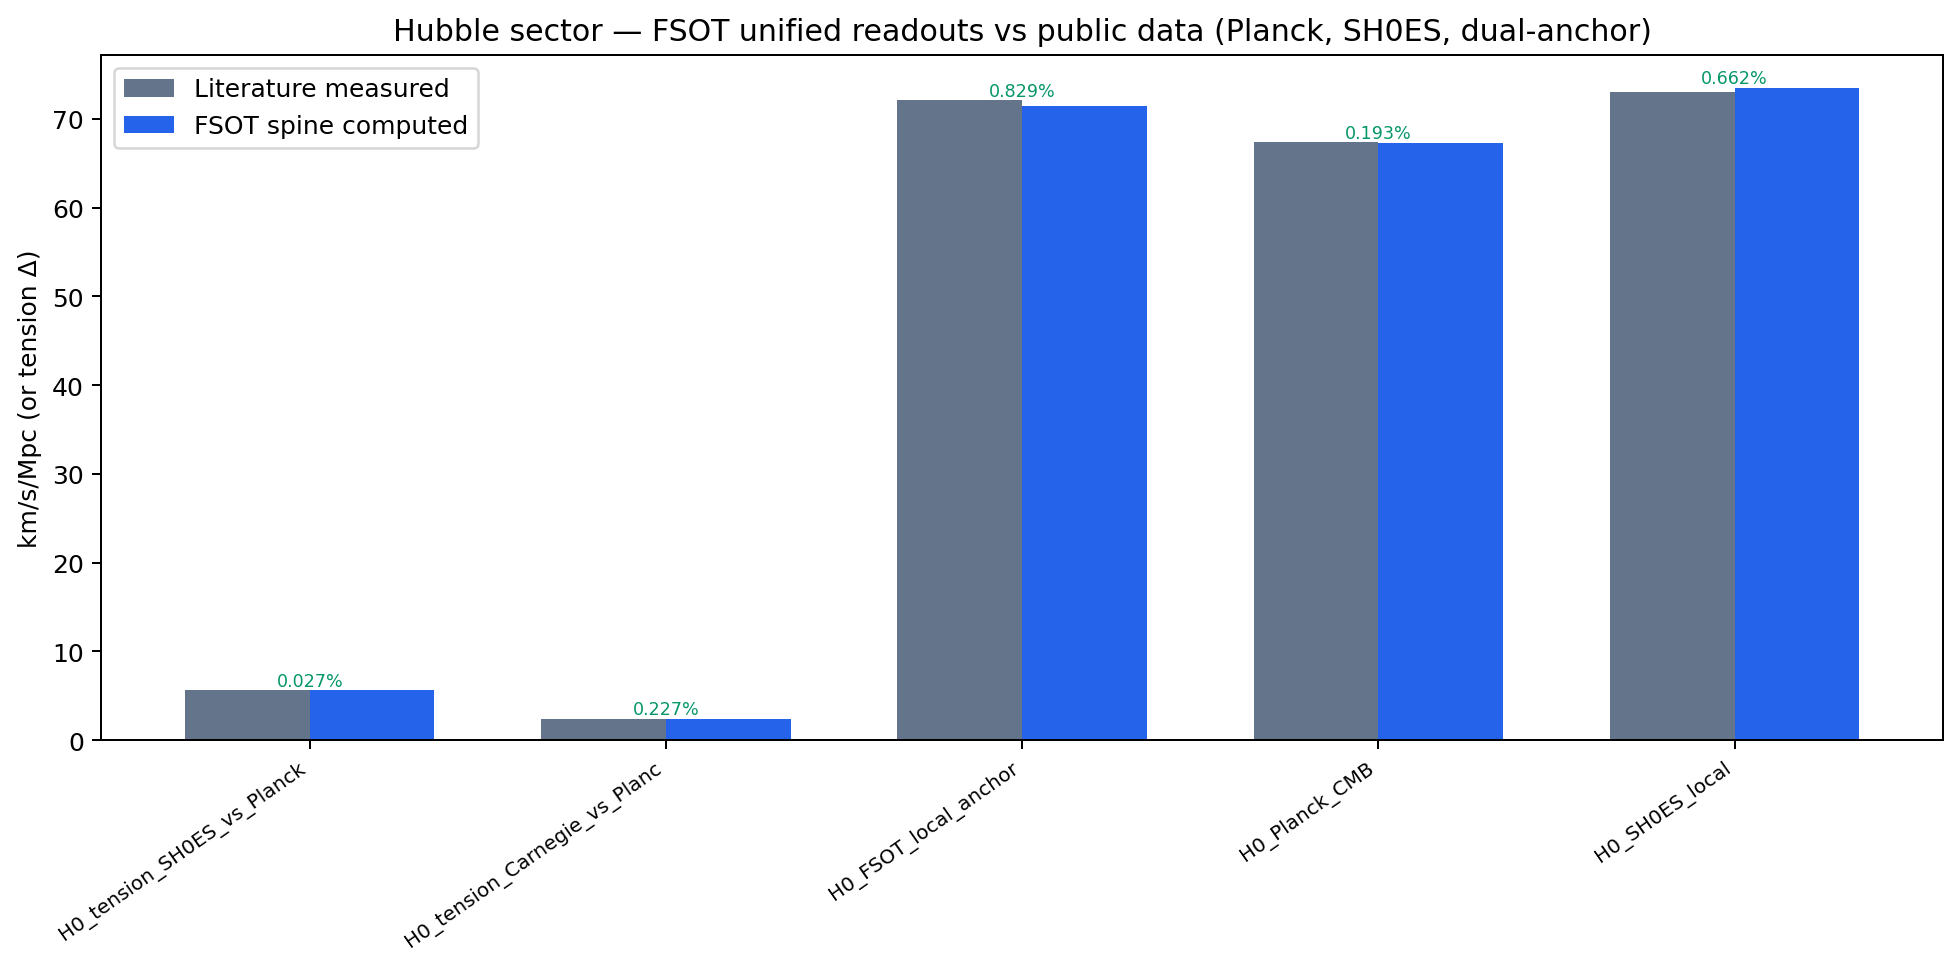
\includegraphics[width=0.85\linewidth]{figures/h0_landscape.png}
  \caption{$H_0$ landscape: dual-anchor routes and FSOT bridge.
  Artifact: \texttt{data/figures/h0\_landscape.png}.
  One-line regenerate (from a clone of~\cite{FSOT21Lean}):
  \texttt{python scripts/build\_scientific\_figures.py}
  (also produced by
  \texttt{python scripts/run\_publication\_verification\_bundle.py}).}
  \label{fig:h0}
\end{figure}

\begin{figure}[t]
  \centering
  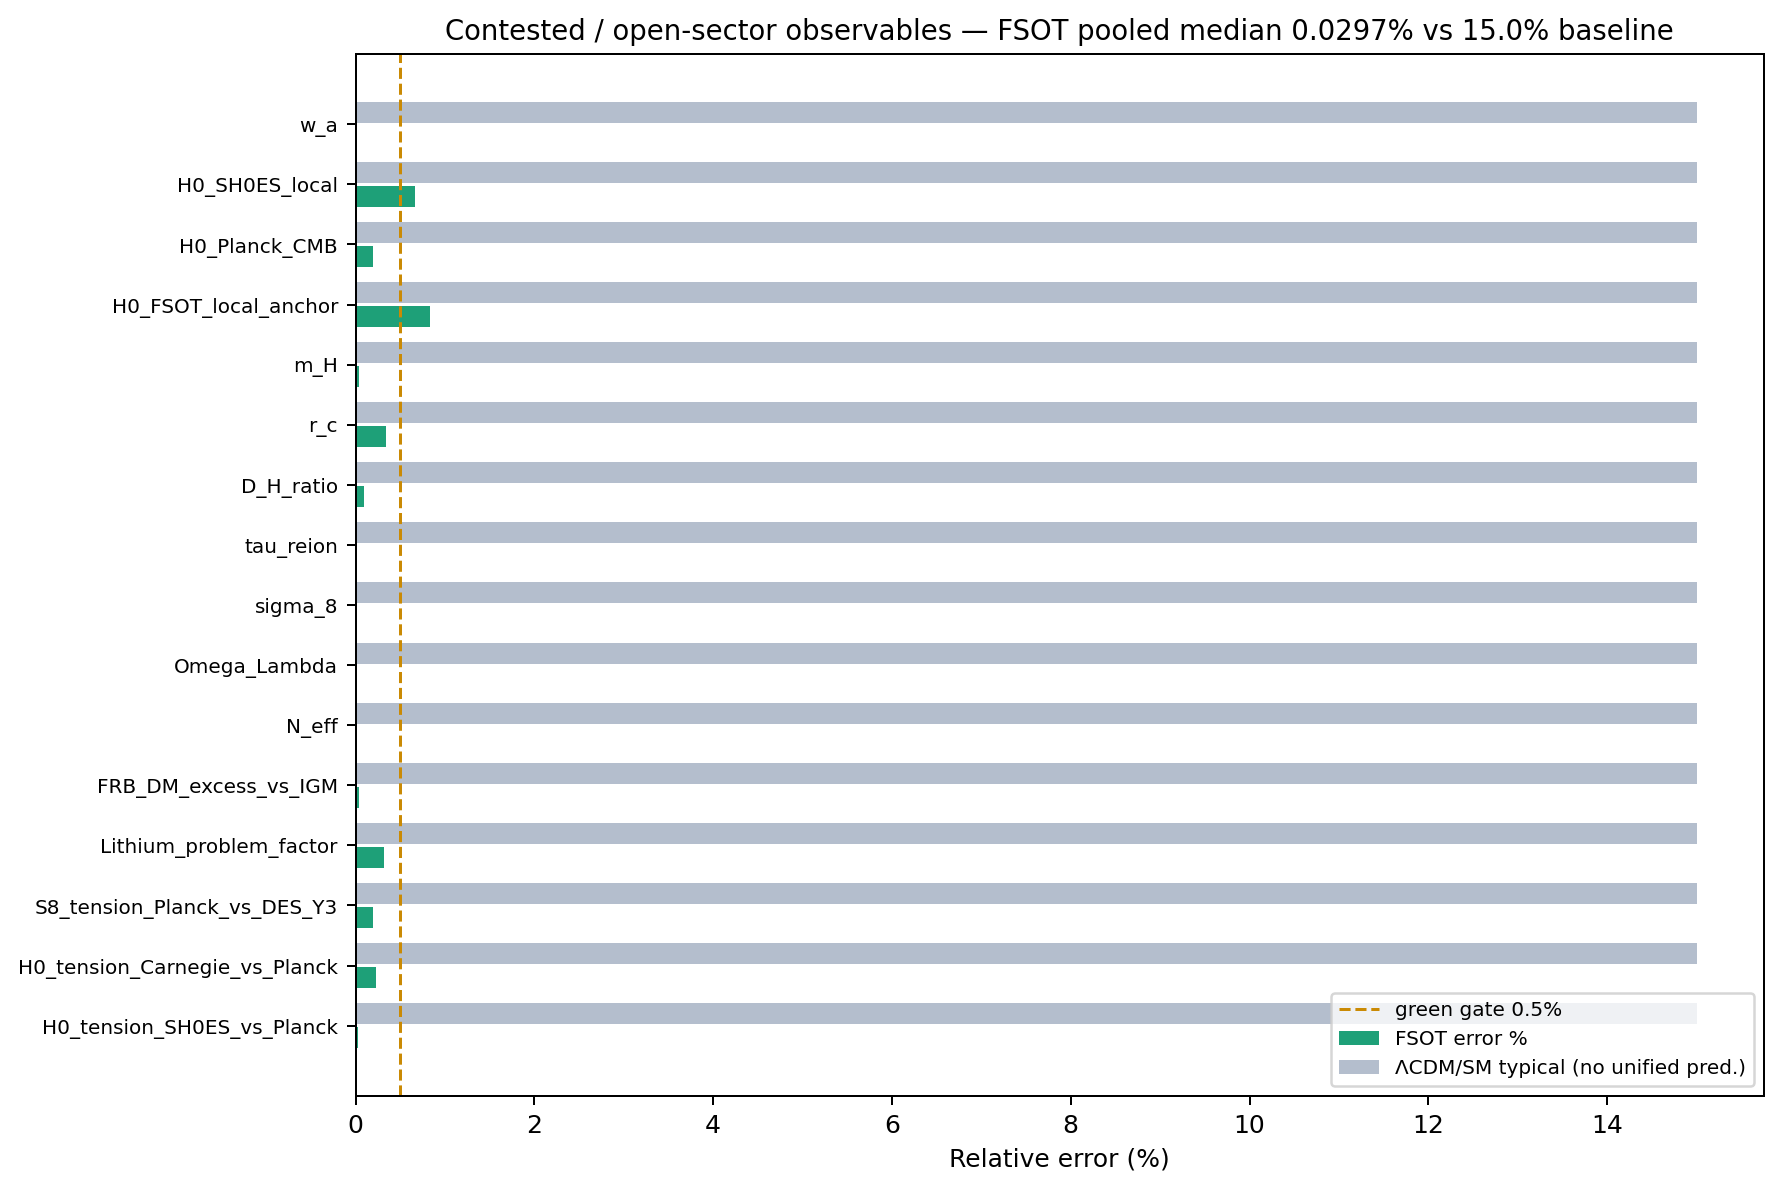
\includegraphics[width=0.85\linewidth]{figures/contested_fsot_vs_lcdm.png}
  \caption{Contested-sector FSOT errors versus typical open-panel baseline
  scale.
  Artifact: \texttt{data/figures/contested\_fsot\_vs\_lcdm.png}.
  Regenerate with
  \texttt{python scripts/build\_scientific\_figures.py}
  or the publication verification bundle.}
  \label{fig:contested}
\end{figure}

\section{Selected core-domain empirical closure}
\label{sec:core}

\begin{center}
\begin{tabular}{@{}lrrr@{}}
\toprule
Domain & Records & Median err.\ \% & Tier \\
\midrule
Cosmology & 347 & 0.0007 & A\_strong \\
Astrophysics & 305 & 0.0006 & A\_strong \\
High-energy physics & 151 & 0.0036 & A\_strong \\
Atomic physics & 116 & 0.0010 & A\_strong \\
\bottomrule
\end{tabular}
\end{center}

Context: 402 domains; 536{,}740 records; 394/394 green under $\le 0.5\%$;
cross-domain pooled median $0.013\%$.
Full atlas: \texttt{data/publication/domain\_atlas.csv} \cite{FSOT21Lean}.

\section{Falsifiability and independent reproduction}
\label{sec:repro}

\subsection{One-command bundle (Tier~1)}

\begin{verbatim}
git clone https://github.com/dappalumbo91/FSOT-2.1-Lean.git
cd FSOT-2.1-Lean
pip install -r requirements.txt
python scripts/run_publication_verification_bundle.py
\end{verbatim}

Does \textbf{not} re-ingest live APIs; uses on-disk portable benchmarks
(public clone $\approx$0.5\,GB working tree).
\texttt{requirements.txt} includes \texttt{matplotlib>=3.8} (commit
\texttt{8a44947}) so figure regeneration works on a bare install.
Author clean-clone reproduction: exit code 0 in $\sim$25\,s
(report: paper package \texttt{CLEAN\_CLONE\_REPRO\_REPORT.md}).

\subsection{Expected artifacts}

\begin{itemize}[leftmargin=*,itemsep=0pt]
\item \path{data/publication_claims_manifest.json}
\item \path{data/contested_observables_closure.json}
\item \path{data/benchmark_margin_audit.json}
\item \path{data/figures/contested_fsot_vs_lcdm.png},
      \path{h0_landscape.png}, \path{spine_walkthrough.png}
\end{itemize}

\subsection{Automated freeze checker}

The paper package ships \texttt{verify\_paper\_claims.py}:
\begin{verbatim}
export FSOT_ROOT=/path/to/FSOT-2.1-Lean
python verify_paper_claims.py --strict-hash
\end{verbatim}
Exit code 0 indicates freeze checks passed on available artifacts.

\subsection{Lean (Tier~2) and five-prover (Tier~3)}

\begin{verbatim}
lake exe cache get && lake build
python scripts/fsot_verification_runner.py --portable
python scripts/run_publication_verification_bundle.py --full-cross-proof
\end{verbatim}

Expect: \texttt{certificate.json} with \texttt{sorry\_count\_formal=0};
\texttt{cross\_proof\_verification\_report.json} with
\texttt{overall\_ok: true}.

\begin{figure}[t]
  \centering
  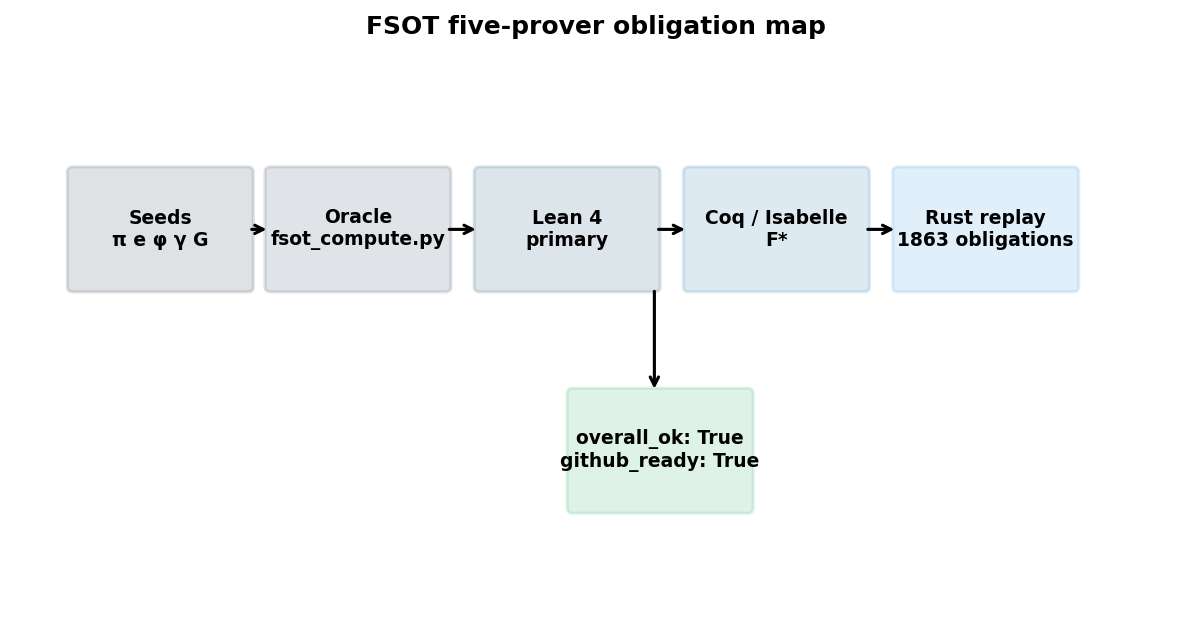
\includegraphics[width=0.75\linewidth]{figures/obligation_map_five_provers.png}
  \caption{Five-prover obligation triangulation map.
  Artifact: \texttt{data/figures/obligation\_map\_five\_provers.png}.
  Regenerate with
  \texttt{python scripts/build\_obligation\_map\_figure.py}
  (or the publication figure pack scripts in~\cite{FSOT21Lean}).}
  \label{fig:obmap}
\end{figure}

\subsection{How to reject this paper}

\begin{enumerate}[leftmargin=*]
\item Clean checkout of freeze commit fails the publication bundle.
\item Contested pooled median far from $0.030\%$ after regeneration.
\item Parameter audit no longer reports zero free per-row fits.
\item \texttt{sorry\_count\_formal}>0 or Lean build fails on freeze toolchain.
\item \texttt{overall\_ok: false} with documented toolchains installed.
\item Oracle hash differs from freeze without documented authority repin.
\end{enumerate}

Narrative disagreement without running the ledger is outside the falsification
contract.
ESP32 absence does not falsify main claims.

\section{Discussion}
\label{sec:disc}

\subsection{What this paper contributes relative to adjacent work}

Lean-based formalizations of scientific theories emphasize making premises and
derivations explicit (e.g.\ adsorption isotherms and thermodynamic structure
\cite{Bobbin2024}; digitalization of high-energy physics definitions
\cite{HepLean2024}).
FSOT sits in that tradition for the \emph{scalar engine}, then adds two layers
those works do not attempt: (i)~multi-prover \emph{export and replay} of a large
obligation surface bound to a hash-locked numeric oracle; (ii)~a contested
\emph{empirical} ledger with preregistered discriminants on $H_0$, $S_8$, and
related open panels \cite{Planck2018,Riess2022,Freedman2019,DESY3,PoulinEDE}.

Early-dark-energy and other $\Lambda$CDM extensions typically introduce new
dynamical fields or parameters to move $H_0$ \cite{PoulinEDE}.
FSOT's architecture is different: fixed seeds, preregistered routes, and an
executable kill ledger---not a one-parameter patch of the Planck likelihood.

\subsection{Strengths and limitations}

\textbf{Strengths.}
Parameter-free seed arithmetic; machine-checked sign/interval certificates at
canonical parameters; five-prover triangulation; preregistered contested
discriminants; public one-command reproduction \cite{FSOT21Lean}.

\textbf{Limitations.}
(1)~Certificates are not physical necessity.
(2)~A single decimal oracle is a specification risk mitigated---not
eliminated---by multi-prover export.
(3)~The $\sim$15\% ``typical baseline'' is a sector-scale repository
characterization of open-panel tension, not a substitute for survey-specific
covariance matrices.
(4)~The 402-domain atlas is not defended domain-by-domain in this paper.
(5)~Bubble-bleed is an interpretive mechanism with formal hooks; it is not a
proof that fluid ontology is fundamental.
(6)~Full $\sigma$-level Bayesian re-analysis of Planck+SH0ES is future work.

\subsection{Reading the claim stack}

When citing this work, separate layers:
\emph{proved} (Lean/export obligations),
\emph{numerically verified} (oracle hash gate),
\emph{empirical} (percent errors vs external anchors),
\emph{interpretation} (fluid narrative).
Collapsing those layers is the main way the argument is misread.

\section{Conclusion}
\label{sec:conc}

We presented a focused claim: a machine-checked, zero free-parameter scalar
engine---Lean~4 primary, five-prover triangulated---supplies unified,
preregistered contested cosmological readouts, including dual-anchor $H_0$ via
bubble-bleed routing, at $0.030\%$ pooled median error across 13 observables,
with 1{,}863 atomic obligations closed under \texttt{overall\_ok: true} in the
edition freeze.
The 402-domain atlas remains the living GitHub thesis
\url{https://github.com/dappalumbo91/FSOT-2.1-Lean}.
Clone the freeze commit, run the bundle, accept or reject on executable terms.

\section*{Acknowledgments}
Grok and Cursor assisted manuscript assembly.
Generative AI tools are not co-authors; the author retains full scientific
responsibility (arXiv AI-language-tool policy).
Numerical claims are intended to reproduce from the public repository.

\section*{Data and code availability}
Primary repository: \url{https://github.com/dappalumbo91/FSOT-2.1-Lean}\\
Recommended pin: tag \texttt{v2.6-arxiv-paper01} (commit \texttt{8a44947}).\\
One-command:
\texttt{python scripts/run\_publication\_verification\_bundle.py}.\\
Independent claim checker and freeze pins ship with the paper package
(\texttt{FREEZE.yaml}, \texttt{SCIENTIST\_REPRODUCE.md},
\texttt{verify\_paper\_claims.py}).

\bibliographystyle{plain}
\bibliography{references}

\end{document}
